% Drawing 31/03-4 -- folder 31, batch 03, archive page 57 (PDF page 58).
% Transcription: à gauche de l'exemple 4, une figure : deux ovales $Y_1$ et $Y_2$ qui se recoupent en deux points, marqués $a$ (en haut) et $b$ (en bas)
% Kind: two overlapping ovals. Method 2 (schematic redraw from the facsimile). Status: ok.
% Notes: Ink (the lower left of Y_1 faint). Two ellipses crossing twice; a above the upper crossing, b below the lower one, Y_1 and Y_2 under the ovals. Redrawn 2026-11-12 (issue 128): to check again.
% Coordinates: 1 unit = 1 mm = 1/100 of the crop width (bbox in page fractions: [0.12, 0.2, 0.5, 0.37]).
% Redrawn by Claude (claude-fable-5-2), issue #128, 2026-11-12; not checked by a human; not compiled (no TeX in the session).
% Rights: reproduces part of the work -- behind RENDER_TRANSCRIPTS, never published by itself.
\documentclass[tikz,border=3pt]{standalone}
\usepackage{amsmath,amssymb}
\usetikzlibrary{patterns,arrows.meta}
\tikzset{pencil/.style={black!45}, struck/.style={black!35}, mpt/.style={circle,draw,inner sep=1.3pt}, pt/.style={circle,fill,inner sep=0.9pt}, opt/.style={circle,draw,fill=white,inner sep=1.1pt}}
\begin{document}
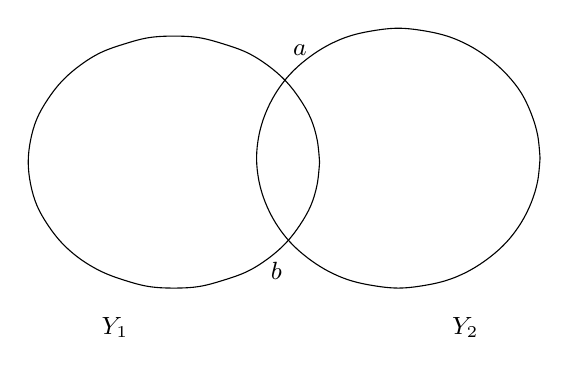
\begin{tikzpicture}[x=1mm,y=1mm,line cap=round,line join=round,font=\scriptsize]
\draw plot[smooth, tension=0.6] coordinates {(48,-30.5) (47.7,-33.3) (46.9,-36) (45.5,-38.5) (43.7,-40.8) (41.4,-42.8) (38.8,-44.4) (35.8,-45.5) (32.7,-46.3) (29.5,-46.5) (26.3,-46.3) (23.2,-45.5) (20.3,-44.4) (17.6,-42.8) (15.3,-40.8) (13.5,-38.5) (12.1,-36) (11.3,-33.3) (11,-30.5) (11.3,-27.7) (12.1,-25) (13.5,-22.5) (15.3,-20.2) (17.6,-18.2) (20.2,-16.6) (23.2,-15.5) (26.3,-14.7) (29.5,-14.5) (32.7,-14.7) (35.8,-15.5) (38.8,-16.6) (41.4,-18.2) (43.7,-20.2) (45.5,-22.5) (46.9,-25) (47.7,-27.7) (48,-30.5)};
\draw plot[smooth, tension=0.6] coordinates {(76,-30) (75.7,-32.9) (74.9,-35.6) (73.6,-38.2) (71.8,-40.6) (69.6,-42.6) (67,-44.3) (64.2,-45.5) (61.1,-46.2) (58,-46.5) (54.9,-46.2) (51.8,-45.5) (49,-44.3) (46.4,-42.6) (44.2,-40.6) (42.4,-38.2) (41.1,-35.6) (40.3,-32.9) (40,-30) (40.3,-27.1) (41.1,-24.4) (42.4,-21.8) (44.2,-19.4) (46.4,-17.4) (49,-15.7) (51.8,-14.5) (54.9,-13.8) (58,-13.5) (61.1,-13.8) (64.2,-14.5) (67,-15.7) (69.6,-17.4) (71.8,-19.4) (73.6,-21.7) (74.9,-24.4) (75.7,-27.1) (76,-30)};
\node[inner sep=1pt] at (45.5,-16.3) {\small $a$};
\node[inner sep=1pt] at (42.5,-44.3) {\small $b$};
\node[inner sep=1pt] at (22,-51.5) {\small $Y_1$};
\node[inner sep=1pt] at (66.5,-51.5) {\small $Y_2$};
\end{tikzpicture}
\end{document}
